\chapter{Schleifen} \label{chp:loops}
\epigraph{You spin me right round, baby // Right round like a record, baby // Right round round round}
{Dead Or Alive}

Computer können dazu benutzt werden, die immer gleichen Aufgaben wiederholt und in schneller Folge auszuführen. Es ist möglich, bei jeder Wiederholung einen einzelnen Eingabewert zu ändern und so \eg Berechnungen für einen ganzen Wertebereich durchzuführen, oder Messwerte von einem Gerät zu überwachen.

Zeichnet man ein \emph{Flussdiagramm} eines solchen Programms (wie in Abbildung \ref{fig:FlowBasicLoop}), so findet sich in der Regel ein Programmteil, der zur Vorbereitung dient und in gewohnter Weise \enquote{von oben nach unten} abgearbeitet wird. An diesen schließt sich ein Abschnitt an, der einige Male wiederholt werden soll, und daher im Flussdiagramm als Bogen dargestellt wird. Nach diesem Teil könnte die Ausgabe der Ergebnisse stattfinden, die wiederum in gewohnter \emph{linearer} Weise (also von oben nach unten) bearbeitet wird.

Die Form dieses Flussdiagramms motiviert den Namen \emph{Schleife} für eine solche Struktur.

\begin{figure}[h!]
\begin{center}
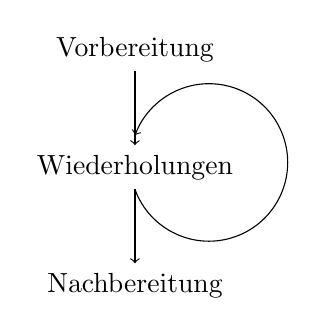
\begin{tikzpicture}
    \node at (0, 3  ) (Input)      {Vorbereitung};
    \node at (0, 1.5) (Operations) {Wiederholungen};
    \node at (0, 0  ) (Output)     {Nachbereitung};

    \draw [->] (Input) -- (Operations);
    \draw [->] (Operations.south)arc(-160:160:1.0);		%start angle: stop angle : radius
    \draw [->] (Operations) -- (Output);
\end{tikzpicture}
\caption{Programmflussdiagramm mit Schleife} \label{fig:FlowBasicLoop}
\end{center}
\end{figure}

In der Regel ist die Zahl der Schleifendurchläufe an eine Bedingung geknüpft; genauso sind aber auch \emph{Endlosschleifen} möglich. In diesem Kapitel werden wir verschiedene Schleifentypen und ihre Anwendungsfelder kennen lernen.

\begin{hintbox}[Laufende Programme zum Beenden zwingen: \texttt{STRG + C}]
Macht man einen Fehler bei der Formulierung der Bedingung, so kann man unbeabsichtigt eine Endlosschleife erstellen. Ein solches Programm wird von sich selbst aus nie beendet. Wir können zu jeder Zeit aber das Beenden erzwingen, indem wir in der Konsole die Tastenkombination \texttt{STRG + C} drücken.
\end{hintbox}

\section{Programmsprünge: \mintinline{c}{goto}}
Die einfachste Form, Schleifen zu implementieren, lässt sich mit der \emph{Sprunganweisung} \mintinline{c}{goto} realisieren. Stellen wir uns vor, der Computer würde mit einem Cursor durch unser Programm laufen und Zeile für Zeile bearbeiten, so ist \mintinline{c}{goto} der Befehl, den Cursor an eine bestimmte Stelle zu verschieben. Sprünge sind sowohl vorwärts als auch rückwärts möglich.

Für einen Sprung ist zunächst eine \emph{Sprungmarke} nötig, also ein Punkt, ab der das Programm fortgeführt wird. Eine solche Sprungmarke hat einen Namen, der denselben Regeln folgt, wie Variablennamen (darf nur einmal im Programm vorkommen; Unterscheidung von Groß- und Kleinschreibung; nur alphanumerische Zeichen; darf nicht mit einer Zahl beginnen; maximal 40 Zeichen lang). Im Code wird sie durch einen Doppelpunkt abgeschlossen.

Der Sprung selbst folgt dann der Syntax:
\begin{codebox}[Syntax: \texttt{goto}]
\begin{minted}{c}
goto Sprungmarke;
\end{minted}
\end{codebox}

Hier sehen Sie ein einfaches Anwendungsbeispiel:
\begin{codebox}[Beispiel: Sprünge mit \texttt{goto}]
\begin{minted}[linenos]{c}
#include <stdio.h>

int main () {
   printf("Erste Zeile der Ausgabe.\n");
   goto ReEntryPoint;

   printf("Dies wird nie ausgegeben.\n");

   ReEntryPoint:
   printf("Letzte Zeile der Ausgabe.\n");
}
\end{minted}
\end{codebox}

Nach der Ausgabe in Zeile 4 springt der \enquote{Cursor} weiter zu Zeile 9. Aller Code dazwischen wird nie ausgeführt. Die Ausgabe lautet entsprechend:

\begin{cmdbox}[Ausführungsbeispiel: Sprünge mit \texttt{goto}]
\begin{minted}{text}
Erste Zeile der Ausgabe.
Letzte Zeile der Ausgabe.
\end{minted}
\end{cmdbox}

Wir können Sprünge mit \mintinline{c}{if} an eine Bedingung knüpfen und so eine Schleife erzeugen, die auch wieder verlassen wird:

\begin{codebox}[Beispiel: Quadratwurzeln der Zahlen 1 bis 10 mit \texttt{goto}]
\begin{minted}[linenos]{c}
#include <stdio.h>
#include <math.h>

int main () {
   double foo = 1;
\end{minted}
\end{codebox}
%
\begin{codebox}[]
\begin{minted}[linenos, firstnumber=last]{c}
   iterationPoint:
   printf("Die Wurzel aus %4.1lf ist %lf.\n", foo, sqrt(foo));
   foo++;

   if (foo <= 10) {goto iterationPoint;}

   printf("Erfolgreicher Programmabschluss.\n");
}
\end{minted}
\end{codebox}

\begin{cmdbox}[Ausführungsbeispiel: Quadratwurzeln der Zahlen 1 bis 10 mit \texttt{goto}]
\begin{minted}{text}
Die Wurzel aus  1.0 ist 1.000000.
Die Wurzel aus  2.0 ist 1.414214.
Die Wurzel aus  3.0 ist 1.732051.
Die Wurzel aus  4.0 ist 2.000000.
Die Wurzel aus  5.0 ist 2.236068.
Die Wurzel aus  6.0 ist 2.449490.
Die Wurzel aus  7.0 ist 2.645751.
Die Wurzel aus  8.0 ist 2.828427.
Die Wurzel aus  9.0 ist 3.000000.
Die Wurzel aus 10.0 ist 3.162278.
Erfolgreicher Programmabschluss.
\end{minted}
\end{cmdbox}

\begin{warnbox}[Spaghetti-Code]
Was Sie gerade über \mintinline{c}{goto} gehört haben, dient vor allem dem besseren Verständnis der folgenden Schleifentypen. Programme, die viele \mintinline{c}{goto}-Sprunganweisungen enthalten werden schnell unübersichtlich. Die einzelnen \enquote{Fäden} des Programmes kreuzen sich und laufen durcheinander wie Spaghetti auf einem Teller. Es wird schwierig, den Programmfluss zu verfolgen und Fehler sammeln sich an.

Die folgenden Schleifentypen sind für Menschen besser zu bedienen, werden aber vom Compiler ebenso in \mintinline{c}{goto}-Programmsprünge umgesetzt.

Es ist prinzipiell immer möglich, ohne den Befehl \mintinline{c}{goto} auszukommen und in den weit meisten Fällen auch zu bevorzugen. ProgrammiererInnen diskutieren kontrovers, ob der Befehl aus dem Sprachumfang der Sprache C (oder damit verwandten Sprachen) gestrichen werden sollte. In Abschnitt \ref{sec:ControlFluxAdjustment} werden Sie allerdings einen Fall sehen, wo \mintinline{c}{goto} tatsächlich eine \emph{elegantere} Lösung darstellt, als die Alternativen.
\end{warnbox}

\section{Schleife mit Bedingung: \mintinline{c}{while}}
Das Schlüsselwort \mintinline{c}{while} lehnt sich an den Sprachgebrauch an, und implementiert die Idee: FALLS \emph{Bedingung erfüllt} WIEDERHOLE \emph{Anweisungen}. Dabei ist \emph{Bedingung} ein Ausdruck wie schon bei \mintinline{c}{if}, der zu einem Wahrheitswert ausgewertet werden kann. Die Syntax lautet:

\begin{codebox}[Syntax: \texttt{while}]
\begin{minted}{c}
while (Bedingung) {
   Anweisungen;
}
\end{minted}
\end{codebox}

Mit diesem Schlüsselwort übersetzt sich also das vorige Beispiel zu folgendem Code:

\begin{codebox}[Beispiel: Quadratwurzeln der Zahlen 1 bis 10 mit \texttt{while}]
\begin{minted}[linenos]{c}
#include <stdio.h>
#include <math.h>

int main () {
   double foo = 1;

   while (foo <= 10) {
      printf("Die Wurzel aus %4.1lf ist %lf.\n", foo, sqrt(foo));
      foo++;
   }

   printf("Erfolgreicher Programmabschluss.\n");
}
\end{minted}
\end{codebox}

Wie schon bei \mintinline{c}{if} können bei einzeiligen Anweisungsblocks die \{geschweiften Klammern\} entfallen. Genauso wie bei \mintinline{c}{if}-Blocks empfehle ich bei Schleifen immer Klammern zu setzen.

Die Bedingung wird bereits vor Eintritt in die Schleife überprüft. Ist sie vor dem Eintritt nicht erfüllt, wird der Schleifen-Körper nie ausgeführt sondern komplett übersprungen.

\begin{hintbox}[Absichtliche Endlosschleife]
Es gibt Situationen, in denen eine Schleife bewusst endlos lange laufen soll, \eg um ein Gerät zu überwachen, das nie abgeschalten wird, oder weil andere Mechanismen das Verlassen der Schleife bewirken können. Für diesen Fall setzt man für gewöhnlich einfach
\begin{center}
\mintinline{c}{while (1)}
\end{center}
Die Konstante \texttt{1} kann sich nicht ändern und entspricht direkt dem Wahrheitswert \emph{true}.
\end{hintbox}

\section{Schleife mit Bedingung und einem garantierten Durchlauf: \mintinline{c}{do-while}}
Schleifen mit dem Konstrukt \mintinline{c}{do-while} funktionieren nach demselben Prinzip wie \mintinline{c}{while}-Schleifen. Allerdings findet die Prüfung der Bedingung erst \emph{am Ende der Schleife} statt, und nicht schon vor Eintritt in die Schleife. Dies bewirkt, dass der Schleifenkörper mindestens einmal durchlaufen wird.

Die Syntax ist sehr ähnlich der von \mintinline{c}{while}:
\begin{codebox}[Syntax: \texttt{do-while}]
\begin{minted}{c}
do {
   Anweisungen;
} while (Bedingung);
\end{minted}
\end{codebox}

Die folgenden beiden Beispiele und Ausgaben verdeutlichen den Unterschied:
\begin{tcbraster}[raster columns=2,
                  raster equal height,
                  nobeforeafter,
                  raster column skip=0.5cm]
\begin{codebox}[Schleife mit \texttt{while}]
\begin{minted}[linenos]{c}
#include <stdio.h>

int main () {
   unsigned int foo = 0;

   while (foo > 0) {
      printf("Schleifenkörper.\n");
   }

   printf("Programmende.\n");
}
\end{minted}
\end{codebox}
%
\begin{codebox}[Schleife mit \texttt{do-while}]
\begin{minted}[linenos]{c}

#include <stdio.h>

int main () {
   unsigned int foo = 0;

   do {
      printf("Schleifenkörper.\n");
   } while (foo > 0);

   printf("Programmende.\n");
}
\end{minted}
\end{codebox}
\end{tcbraster}

In beiden Fällen ist die Bedingung \texttt{foo > 0} zu keiner Zeit erfüllt. Dennoch sind die beiden Ausgaben unterschiedlich:

\begin{tcbraster}[raster columns=2,
                  raster equal height,
                  nobeforeafter,
                  raster column skip=0.5cm]
\begin{cmdbox}[Ausführungsbeispiel: Schleife mit \texttt{while}]
\begin{minted}{text}
Programmende.
\end{minted}
\end{cmdbox}
%
\begin{cmdbox}[Ausführungsbeispiel: Schleife mit do-while]
\begin{minted}{text}
Schleifenkörper.
Programmende.
\end{minted}
\end{cmdbox}
\end{tcbraster}

Die \mintinline{c}{do-while}-Schleife kommt also zum Einsatz wenn der Schleifenkörper garantiert \emph{mindestens einmal} ausgeführt werden soll.

\section{Zählschleifen: \mintinline{c}{for}}
Der Schleifen-Typ \mintinline{c}{while} ist generell für alle Szenarios geeignet. Das häufigste Szenario ist der Fall, in dem eine Variable für jede \emph{Iteration} (\ie für jeden Durchlauf der Schleife) hochgezählt wird. Zu diesem Zweck existiert die spezielle Form der \mintinline{c}{for}-Schleife, die eine kompakte Form solcher Konstrukte erlaubt.

Eine \mintinline{c}{for}-Schleife hat die folgende Form:
\begin{codebox}[Syntax: \texttt{for}]
\begin{minted}{c}
for (Startanweisung; Bedingung; Iteration) {
   Anweisungen;
}
\end{minted}
\end{codebox}

Wobei \texttt{Startanweisung} und \texttt{Iteration} jeweils reguläre C-Anweisungen sind und \texttt{Bedingung} ein Ausdruck, der zu einem Wahrheitswert ausgewertet werden kann. Diese Struktur wird genauso umgesetzt, als würde eine \mintinline{c}{while}-Schleife folgender Form programmiert:

\begin{codebox}[Äquivalente Form mit \texttt{while}]
\begin{minted}{c}
Startanweisung;
while (Bedingung) {
   Anweisungen;
   Iteration;
}
\end{minted}
\end{codebox}

Das heißt, \texttt{Startanweisung} wird automatisch vor Schleifenbeginn und \texttt{Iteration} am Ende jedes Schleifendurchlaufs ausgeführt. In der Regel ist \texttt{Startanweisung} die Zuweisung eines Startwerts zu einer \emph{Zählvariablen}. Mit \texttt{Iteration} wird diese Zählvariable dann hochgezählt (oder in geeigneten Schritten verändert). Üblicherweise wird die \texttt{Bedingung} durch einen Vergleich der Zählvariable mit einem konstanten Wert oder einer Variable realisiert.

Das vorige Beispiel der Quadratwurzeln bis 10 schreibt sich damit folgendermaßen:

\begin{codebox}[Beispiel: Quadratwurzeln der Zahlen 1 bis 10 mit \texttt{for}]
\begin{minted}[linenos]{c}
#include <stdio.h>
#include <math.h>

int main () {
   double foo;

   for (foo = 1; foo <= 10; foo++) {
      printf("Die Wurzel aus %4.1lf ist %lf.\n", foo, sqrt(foo));
   }

   printf("Erfolgreicher Programmabschluss.\n");
}
\end{minted}
\end{codebox}

Mit dem Standard C99 wurde auch die Möglichkeit eingeführt, in \texttt{Startanweisung} Variablen (plural) zu deklarieren und zu initialisieren. Diese \enquote{existieren} dann allerdings nur innerhalb des Schleifenkörpers und können nach Ende der Schleife nicht mehr verwendet werden (es dürfen jedoch nach der Schleife \emph{neue} Variablen mit demselben Namen angelegt werden). Wir werden in Abschnitt \ref{sec:Scopes} mehr hierzu erfahren. Das folgende Beispiel zeigt diese kombinierte Deklaration und Initialisierung:

\begin{codebox}[Beispiel: \texttt{for}-Schleife mit Deklaration]
\begin{minted}[linenos]{c}
#include <stdio.h>
#include <math.h>

int main () {
   for (double foo = 1; foo <= 10; foo++) {
      printf("Die Wurzel aus %4.1lf ist %lf.\n", foo, sqrt(foo));
   }

   printf("Erfolgreicher Programmabschluss.\n");
}
\end{minted}
\end{codebox}

\section{Eingriffe in den Kontrollfluss: \mintinline{c}{break} und \mintinline{c}{continue}} \label{sec:ControlFluxAdjustment}
Es gibt Situationen, in denen eine Schleifen-Ausführung \enquote{vorzeitig} abgebrochen oder ein Teil des Schleifenkörpers \enquote{übersprungen} werden soll. Zu diesem Zweck dienen die Befehle \mintinline{c}{break} und \mintinline{c}{continue}.

Wir kennen \mintinline{c}{break} bereits von \mintinline{c}{switch}-Blöcken. Dort wurden sie benutzt, um den aktuellen \mintinline{c}{switch}-Block zu verlassen und mit der Programmausführung an das Ende des Blocks zu springen. Dieselbe Wirkung hat \mintinline{c}{break} auch bei Schleifen, gleich ob es sich dabei um \mintinline{c}{for}, \mintinline{c}{while} oder \mintinline{c}{do-while} handelt.

Das folgende Beispiel zeigt die Ausgabe von Zahlen und deren Quadrat. Es sollen maximal 100 Zahlen ausgegeben werden, die Ausgabe soll aber stoppen, wenn eine Quadratzahl größer als 1000 ist. Um den bedingten Abbruch der Schleife zu realisieren verwenden wir \mintinline{c}{break}\footnote{Natürlich kann dazu auch ein logisches OR benutzt werden; hier soll aber die Anwendung von \mintinline{c}{break} illustriert werden.}.

\begin{codebox}[Beispiel: Abbruch einer \texttt{for}-Schleife mit \texttt{break}]
\begin{minted}[linenos]{c}
#include <stdio.h>

int main () {
   for (int foo = 1; foo <= 100; foo++) {
      printf("%d -> %d.\n", foo, foo * foo);
      if (foo * foo > 1000) {break;}
   }
}
\end{minted}
\end{codebox}

Die Zahlen 1 bis 32 sowie ihre Quadrate (1 bis 1024) werden ausgegeben, bevor die Schleife durch  \mintinline{c}{break} verlassen wird und die Ausgabe stoppt.

\mintinline{c}{continue} greift ähnlich in die Ausführung ein; jedoch wird die Schleife nicht verlassen sondern die Ausführung springt zum Schleifenbeginn zurück. Bei \mintinline{c}{for}-Schleifen wird zuvor noch \texttt{Iteration} ausgeführt, \ie \eg die Zahlvariable hochgezählt.

Das folgende Beispiel gibt die Zahlen von 1 bis 100 aus mit Ausnahme der durch 5 teilbaren Zahlen:

\begin{codebox}[Beispiel: \texttt{for} mit \texttt{continue}]
\begin{minted}[linenos]{c}
#include <stdio.h>

int main () {
   for (int foo = 1; foo <= 100; foo++) {
      if (foo % 5 == 0) {continue;}
      printf("%d\n", foo);
   }
}
\end{minted}
\end{codebox}
